
\chapter{Rozpoznávání SPZ}

\noindent
Jak již bylo řečeno v kapitole \ref{archtech}, mobilní aplikace pořídí snímek,
pošle ho na Backend, jenž ho pošle serveru s knihovnou OpenALPR, která
rozpozná SPZ a výsledek pošle zpět na backend. V této kapitole si popíšeme
mobilní aplikaci a server s OpenALPR.

\section{Zvyšování přesnosti}

\subsection{Cachování výsledků}

\noindent
Výsledek z knihovny OpenALPR je seznam dvojic udávající SPZ a šanci, že konkrétní SPZ je správně --
jak si OpenALPR věří ve výsledek. Je tudíž logické měření udělat víc a provést aritmetický průměr a
zvolit nejlepší výsledek.

K ukládání takto dočasných dat (přibližně počet měření krát 1 sekunda) se databáze nehodí, a proto
bylo zavedeno ukládání do mezipaměti. V současné chvíli se využívá prostá paměť backendu,
kde klíčem je $id$ zařízení. Díky tomu, že Node.js běží na jednom vlákně, nemusíme se bát souběhu
(angl. race-condition). Externí mezipaměť by bylo vhodné využít (např. Redis), pokud by se spouštělo více
instancí backendu a prováděl by se takzvaný \textit{load-balancing}.

Výchozí počet měření je 2, a lze ho upravit v konfiguraci backendu.

\subsection{Filtrování podle geometrického obsahu}

\noindent
Pokud OpenALPR nalezne SPZ, udá i její pozici ve zdrojovém obrázku.
Aby se tedy předešlo naskenování SPZ, které jsou například daleko, lze odfiltrovat SPZ
podle jejich obsahu v pixelech čtverečních. Konkrétní hodnota je potřeba odladit na místě skenování a
lze změnit ve webové aplikaci pro kterékoliv zařízení.


\section{Autentizace}

\noindent
Zařízení se autentifikuje naskenováním QR kódu, jenž lze najít ve webové aplikaci. Ten obsahuje
JSON řetězec s aktivačním heslem, pomocí kterého se zařízení přihlásí do systému a získa svou konfiguraci.

Samotné skenování QR kódu je provedeno externí aplikací Barcode Scanner od vývojáře
Zxing Team, která lze nainstalovat z Play Store.

Konkrétní mechnismus komunikace s touto externí byl převzán. \citep[viz][]{QrScan}

\section{Volba zařízení pro mobilní aplikaci}

\noindent
Co se týče hardwarového vybavení snímacího zařízení, tak je vyžadována přední kamera
s rozlišením alespoň 1000 na 1000 pixelů. Bližší informace ohledně a zdůvodnění zmenšení jsou v sekci \ref{app_resizing}.
Procesor, RAM i vnitřní paměť může být libovolná -- kterékoliv
dnešní nové zařízení bohatě postačí (za předpokladu, že vnitřní paměť není zaplněná).
Minimální verze Androidu je 5 (SDK 21).

Autorovi se nepodařilo najít způsob, jak zároveň pořizovat v pravidelném intervalu snímky
a mít zařízení uzamknuté proti přístupu. K zajištění pořizování snímků si hlavní
obrazovka aplikace řekně systému Android o zabránění uzamknutí.
To má dva následky. První je, že zařízení by nemělo mít OLED displej, aby nedošlo k takzvanému
\textit{burn-in} \citep[viz][]{OledBurnIn}. Druhý je, že zařízení by mělo být v produkčním provozu
bezpečně uzavřeno v krabičce, nebo by se mělo nacházet na bezpečném místě, aby se předešlo
nepovolené manipulaci.

\section{Životní cyklus mobilní aplikace}

\noindent
Na obrázku \ref{fig:app_lifecycle} lze vidět životní cyklus mobilní aplikace.
Proces neprobíhá na jednom vlákně. Jakmile se pořídí fotografie, tak začně odpočet kolem jedné
sekundy, po kterém se pořídí další, a zároveň se už posílá první fotografie.
Změní-li se konfigurace na backendu, tak je poslána zařízení při dalším kontaktu, jinak
konfigurace poslána není.

\begin{figure}[!htb] \centering
  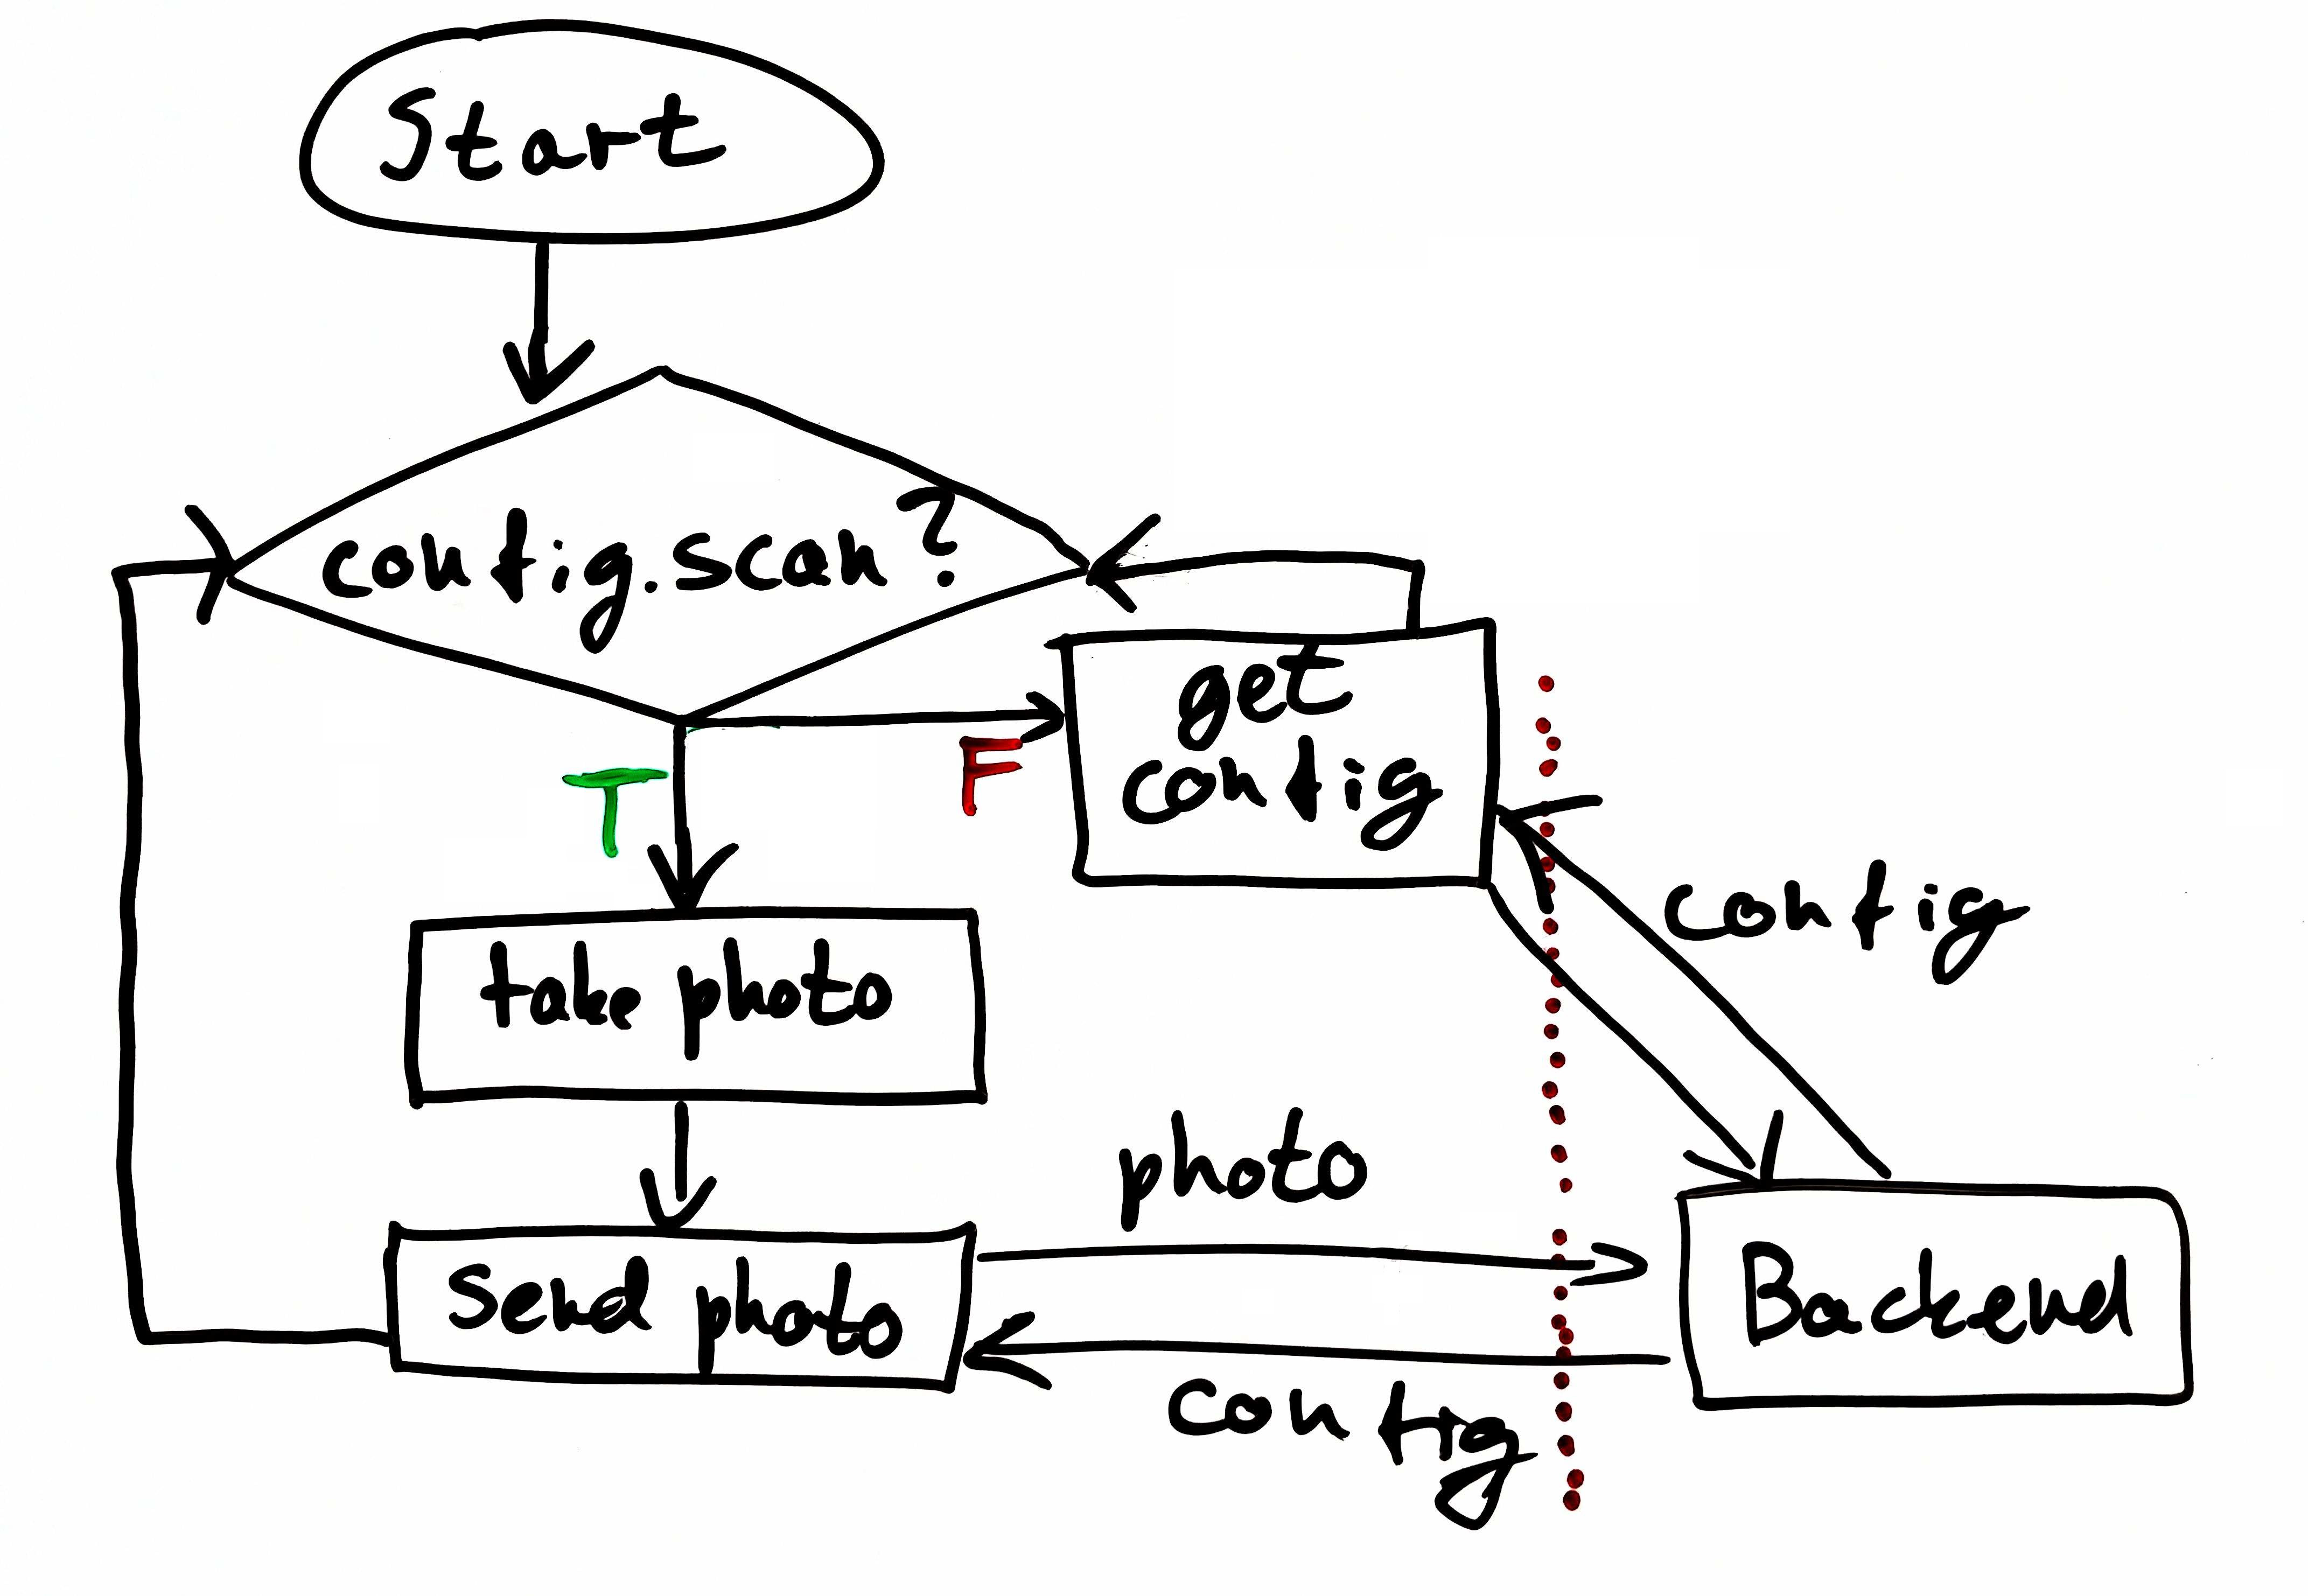
\includegraphics[width=135mm]{../img/app_lifecycle.jpg}
  \caption{Životní cycklus mobilní aplikace.}
  \label{fig:app_lifecycle}
\end{figure}

\section{Optimalizace velikosti přenesených dat} \label{app_resizing}

\noindent
Aby se ušetřilo na přenesených datech a aby rozpoznání proběhlo rychleji,
mobilní aplikace zmenší snímek
na nastavitelnou hodnotu
Tuto funkci poskytuje metoda \textit{createScaledBitmap} v třídě \textit{android.graphics.Bitmap}.

V závislosti na poměru stran snímků největšího rozlišení fotoaparátu,
může být potřeba hodnotu zmenšení změnit.
Základní hodnota je 1300x1000 pixelů, protože aplikace byla testována na
zařízení s fotoaparátem o roslišení 4356x3492 pixelů (poměr stran je 4:3).

Ušetření je opravdu veliké. Při testu s fotoaparátem o rozlišení 4356x3492 pixelů
byla průměrná velikost nezmenšených snímků $1,9$MB (JPG, $N=50$, $\sigma=0,325$).
Průměrná velikost snímků zmenšených na 1300x1000 pixelů byla
$0,15$MB (JPG, $N=50$, $\sigma=0,024$). Kdyby byla frekvence snímání jeden snímek za sekundu,
tak by bez optimalizací byl objem přenesených dat za jeden den $164,16$GB ($3600\cdot24\cdot1,9$MB).
Při stejné frekvenci s optimalizacemi by byl objem přenesených dat za jeden den
$12,96$GB ($3600\cdot24\cdot0,15$MB), což je $7,9$\% objemu bez optimalizací.

\section{Uživatelské rozhraní mobilní aplikace}

\noindent
Uživatelské rozhraní se skládá ze dvou obrazovek. Na obrázcích \ref{fig:app_ui}
lze vidět obě -- hlavní obrazovku a nastavení.

\begin{figure}[!htb] \centering
  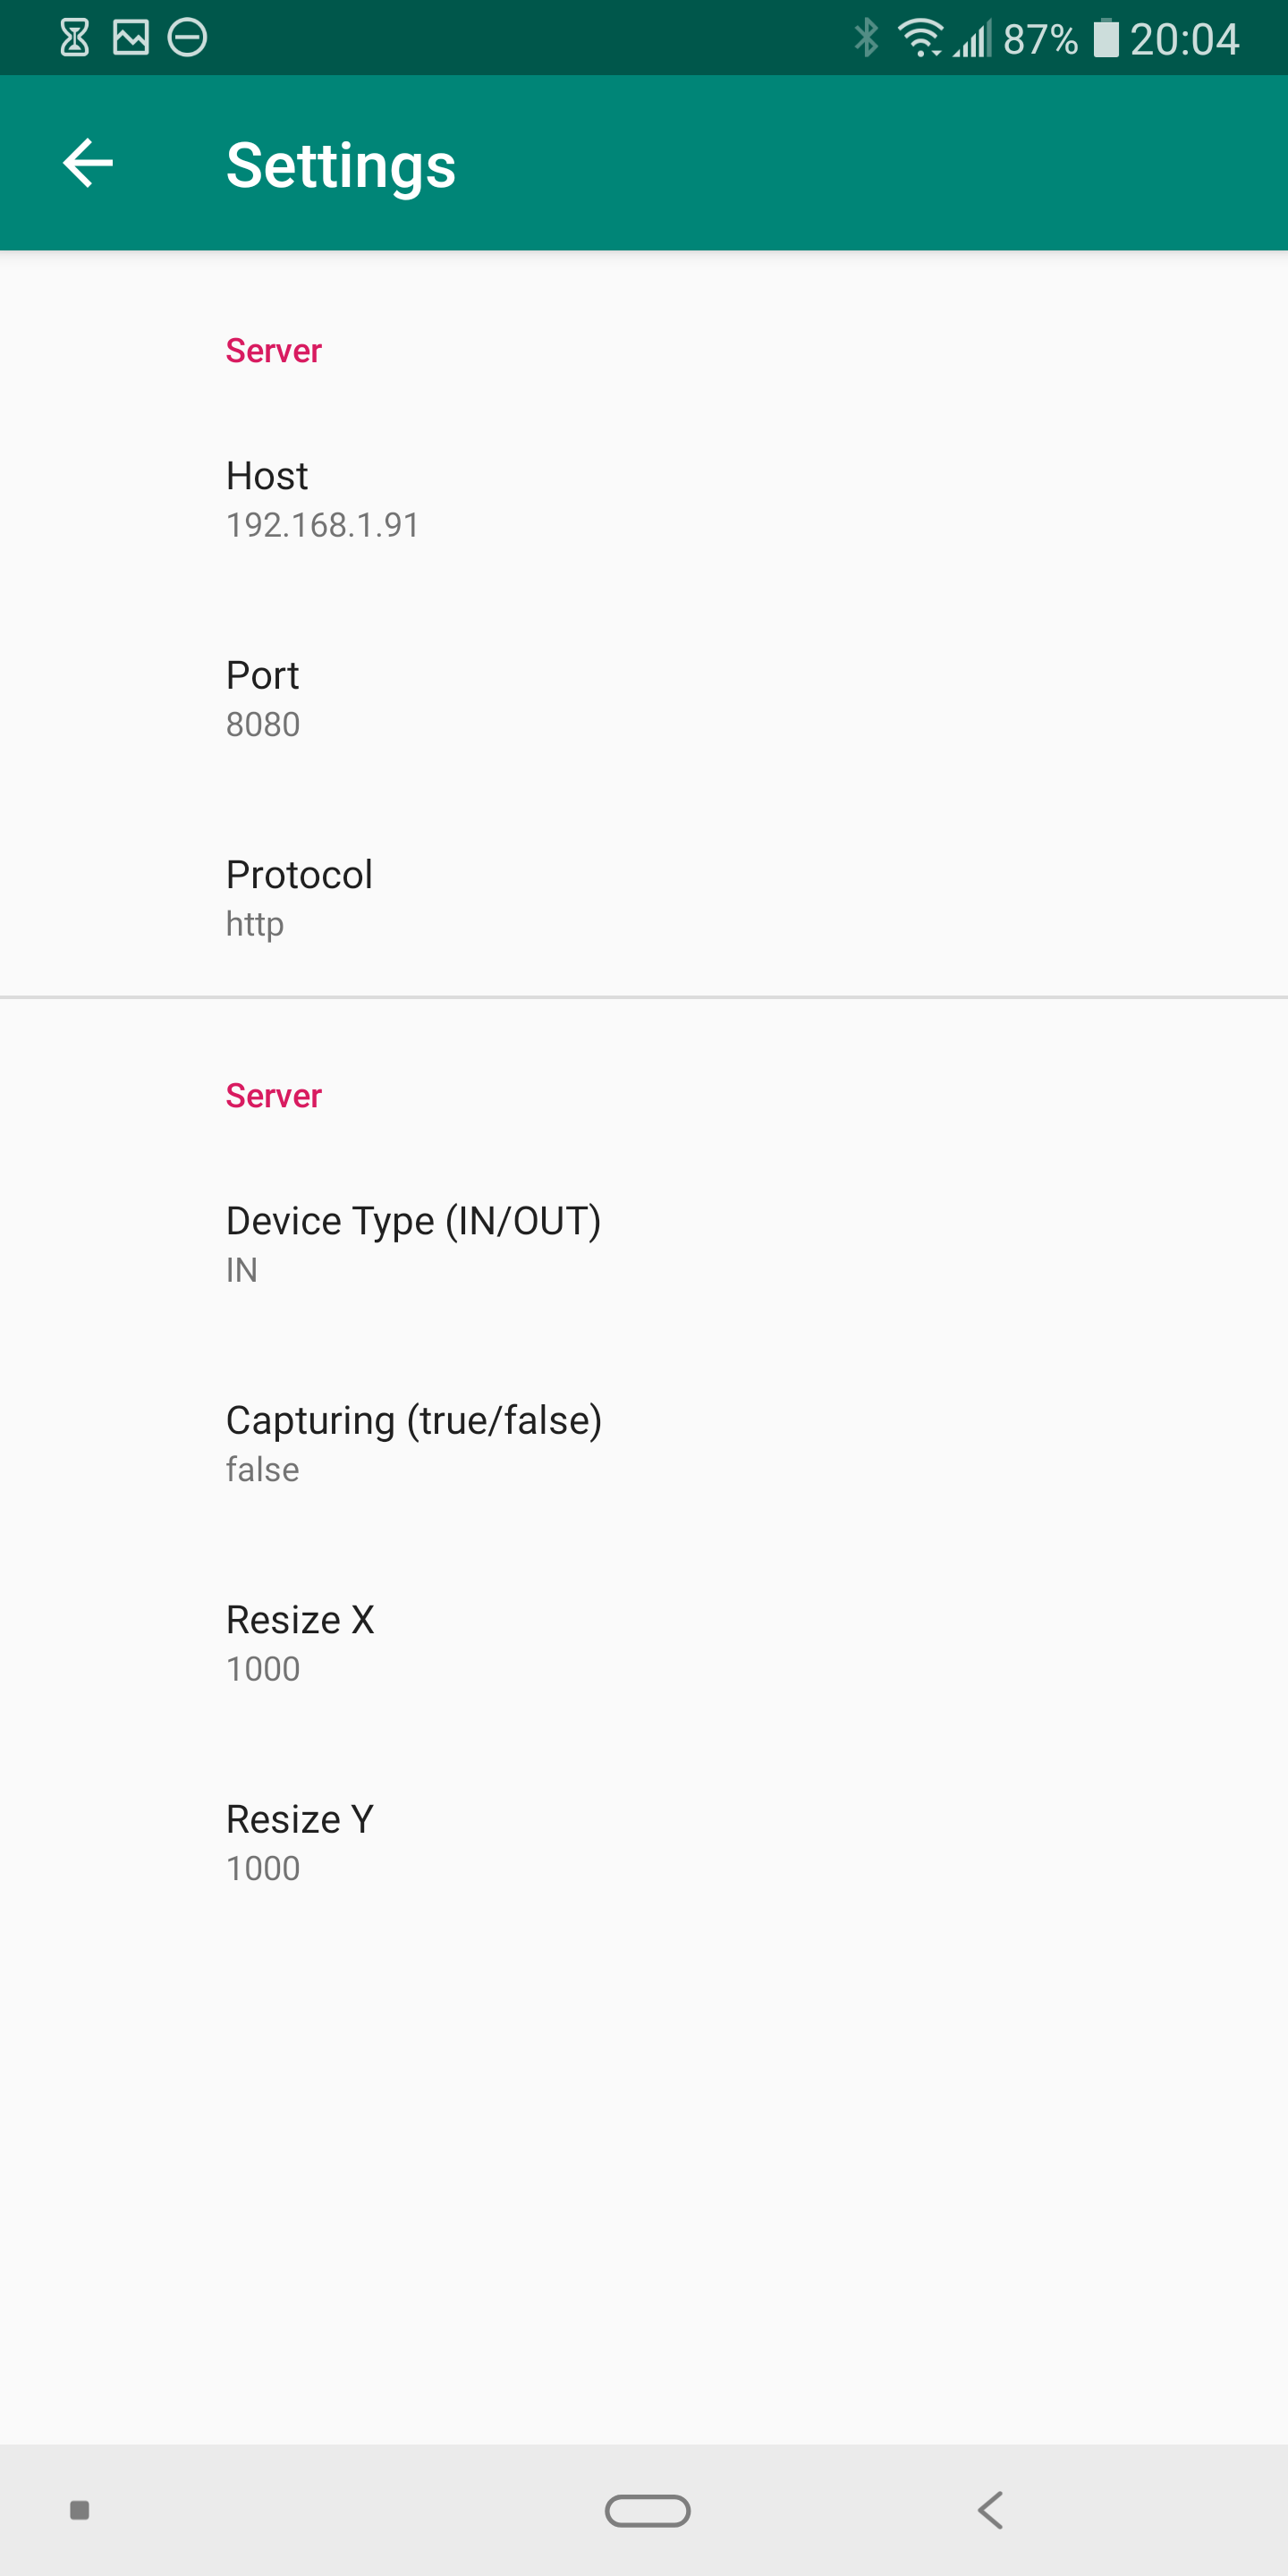
\includegraphics[width=70mm]{../img/app_settings.png}
  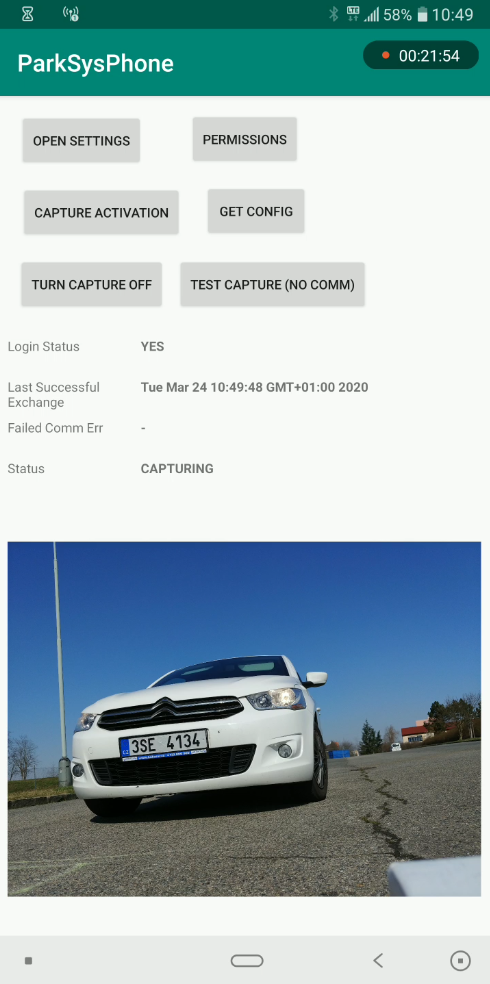
\includegraphics[width=70mm]{../img/app_mainscreen.png}
  \caption{Rozhraní mobilní aplikace.}
  \label{fig:app_ui}
\end{figure}

V nastavení lze nastavit adresu backendu a vybrat si mezi HTTP a HTTPS.

\section{Implementační detaily mobilní aplikace}

\subsection{Komunikace s backendem}

\noindent
Ke komunikaci přes HTTP využívá aplikace knihovnu Volley, která je doporučena
v Android dokumentaci. Princip použití je takový, že si vytvoříme
\textit{singleton} obstarávající frontu žádostí, kterému předáváme HTTP žádosti s
\textit{callback} funkcí obsluhující odpověď. \citep[viz][]{Volley1}

\subsection{Ukládání snímků}

\noindent
Snímky se ukládají do paměti určené pro aplikaci. Kdyby se použily dočasné soubory,
mohlo by se stát, že je systém před posláním nemilosrdně smaže.
\citep[viz][]{AndroidMem}
Aplikace tedy musí obstarávat i mazání souborů, což se provádí
ihned po odeslání snímku na backend.
